\documentclass[border=10pt]{standalone}
\usepackage{tikz}
\usetikzlibrary{shapes.geometric}
\usetikzlibrary{arrows.meta,arrows}
\usepackage{setspace}
\begin{document}
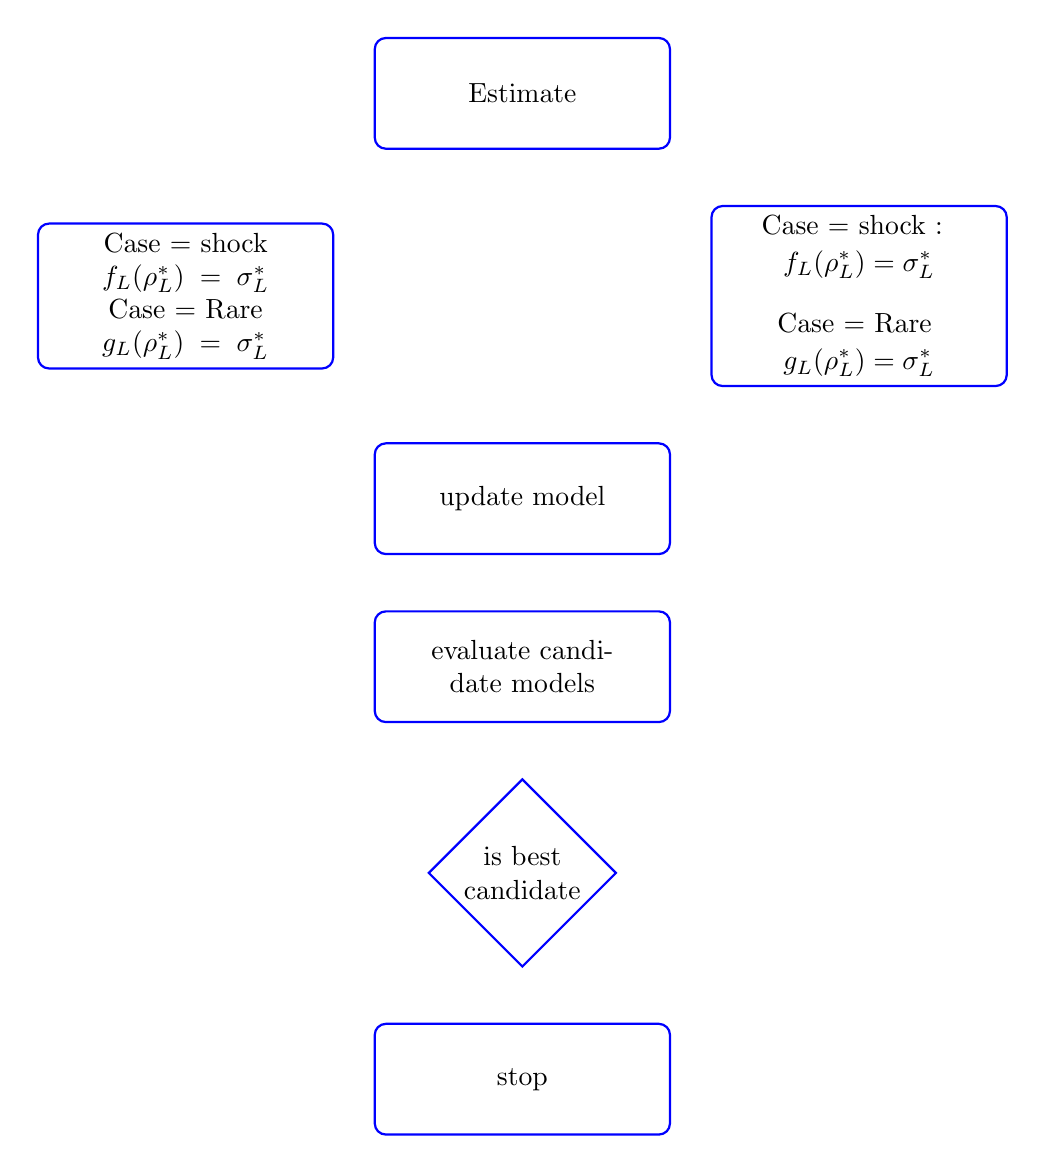
\begin{tikzpicture}
[auto,
decision/.style={diamond, draw=blue, thick,
text width=4.5em,align=flush center,
inner sep=1pt},
block/.style ={rectangle, draw=blue, thick, 
text width=10em,align=center, rounded corners,
minimum height=4em},
line/.style ={draw, thick, -latex',shorten >=2pt},
cloud/.style ={draw=red, thick, ellipse,
minimum height=2em}]
\matrix [column sep=5mm,row sep=7mm]
{
% row 1
& \node [block] (init) {Estimate}; &\\
% row 2
\node [block] (Left) {
Case = shock  $ f_L(\rho_L^*) = \sigma_L^*$ \\  Case = Rare $ g_L(\rho_L^*) = \sigma_L^*$ }; 
&  & \node [block] (Left) {Case = shock : \vspace{-0.3cm}  $$ f_L(\rho_L^*) = \sigma_L^*$$  Case = Rare  \vspace{-0.3cm} $$ g_L(\rho_L^*) = \sigma_L^*$$  }; 
   \\
% row 3
&\node [block] (update) {update model}; &\\
&\node [block] (evaluate) {evaluate candidate models}; & \\
% row 4
& \node [decision] (decide) {is best candidate}; & \\
% row 5
& \node [block] (stop) {stop}; & \\
};
%\begin{scope}[every path/.style=line]
%\path (init) -- (identify);
%\path (identify) -- (evaluate);
%\path (evaluate) -- (decide);
%\path (update) |- (identify);
%\path (decide) -| node [near start] {yes} (update);
%\path (decide) -- node [midway] {no} (stop);
%\path [dashed] (expert) -- (init);
%\path [dashed] (system) -- (init);
%\path [dashed] (system) |- (evaluate);
%\end{scope}
\end{tikzpicture}

\end{document} 
\end{figure}
 \end{document}
